\documentclass[12pt, a4paper]{article}
\usepackage[utf8]{inputenc}
\usepackage[T1]{fontenc}
\usepackage{fontspec}
\usepackage{amsmath}
\usepackage{unicode-math}
\usepackage{amssymb}
\usepackage{graphicx}
\usepackage{geometry}
\usepackage{hyperref}
\usepackage{enumerate}
\usepackage{tabularx}
\usepackage{ragged2e}

\setmainfont{Libertinus Serif}
\setmathfont{Libertinus Math}

% Configuração da geometria da página
\geometry{a4paper, margin=1in}

% Configuração de hiperlinks
\hypersetup{
    colorlinks=true,
    linkcolor=blue,
    filecolor=magenta,      
    urlcolor=cyan,
}

\begin{document}

\title{{\large \textsc{Probabilidade e Estatística}} \\[4pt] {\Huge Prova 3 – Lista}}
\author{}
\date{}
\maketitle

\begin{enumerate}

\item Para verificar o grau de adesão de uma nova cola para vidros, preparam-se dois tipos de montagem; cruzado (A), onde a cola é posta em forma de X, e quadrado (B), onde a fórmula é posta nas 4 bordas. O resultado para a resistência das duas amostras está abaixo. Para um nível de 5\% de significância que tipo de conclusão poderia ser tirada? Antes de fazer o teste de médias, verifique se a pressuposição de variâncias iguais está satisfeita ou não.

\begin{center}
\begin{tabular}{|c|c|}
\hline
\textbf{Método A} & \textbf{Método B} \\
\hline
16 & 13 \\
14 & 19 \\
19 & 14 \\
18 & 17 \\
19 & 21 \\
20 & 24 \\
15 & 10 \\
18 & 14 \\
17 & 13 \\
18 & 15 \\
\hline
\end{tabular}
\end{center}

\item Nas sentenças a seguir, marque V se verdadeiro e F se falso. Caso afirme falso, justifique o motivo de sua decisão.
\begin{enumerate}[a)]
    \item ( ) O teste de hipóteses é um procedimento estatístico onde se busca verificar uma hipótese a respeito da população, tendo por base dados amostrais.
    \item ( ) A hipótese estatística é uma suposição feita a respeito de uma ou mais estatísticas, como, por exemplo a média amostral e a proporção amostral.
    \item ( ) A hipótese nula, supõe a igualdade dos parâmetros que estão sendo comparados.
    \item ( ) Quando não temos motivos suficientes para supor que uma das médias será maior que a outra, formulamos uma hipótese alternativa unilateral (mais genérica).
    \item ( ) Joãozinho Mão Leve foi levado a julgamento. O juiz inocentou Joãozinho, porém ele era culpado. Pensando estatisticamente ($H_0$: culpado), o juiz cometeu, neste caso, o ERRO TIPO I.
    \item ( ) José Inocêncio foi absolvido no julgamento. Ele não havia cometido o delito. Pensando estatisticamente, ($H_0$: inocente), evitou-se o ERRO TIPO II.
    \item ( ) José Inocêncio foi absolvido no julgamento. Ele não havia cometido o delito. Pensando estatisticamente, ($H_0$: culpado), evitou-se o ERRO TIPO II.
    \item ( ) Joãozinho Mão Leve foi levado a julgamento. O juiz inocentou Joãozinho, porém ele era culpado. Pensando estatisticamente ($H_0$: inocente), o juiz cometeu, neste caso, o ERRO TIPO I.
\end{enumerate}

\item Uma pesquisa foi realizada com o objetivo de verificar se existe associação entre a falta de sono e a capacidade de as pessoas resolverem problemas simples. Foram testadas 10 pessoas, mantendo-se sem dormir por um determinado número de horas. Após cada um destes períodos, cada pessoa teve de resolver um teste com adições simples, anotando-se então os erros cometidos. Os dados resultantes são os seguintes:

\begin{center}
\begin{tabular}{|c|c|}
\hline
\textbf{Número de erros} & \textbf{Número de horas sem dormir} \\
\hline
6 & 8 \\
8 & 8 \\
6 & 12 \\
10 & 12 \\
8 & 16 \\
14 & 16 \\
12 & 20 \\
14 & 20 \\
12 & 24 \\
16 & 24 \\
\hline
\end{tabular}
\end{center}

\begin{enumerate}[a)]
    \item Calcule o coeficiente de correlação linear de Pearson, interprete e teste sua significância a 5\%.
    \item Ajuste, teste e interprete o modelo de regressão linear simples.
\end{enumerate}

\item Um experimento mediu o rendimento de trigo em sete diferentes níveis de Nitrogênio, com os seguintes resultados.
\begin{enumerate}[a)]
    \item Calcule o coeficiente de correlação linear de Pearson, interprete e teste sua significância a 5\%.
    \item Ajuste, teste e interprete o modelo de regressão linear simples.
\end{enumerate}

\begin{center}
\begin{tabular}{|c|c|}
\hline
\textbf{Unidades (Kg de $N/ha$)} & \textbf{Rendimento $(t/ha)$} \\
\hline
40 & 15,9 \\
60 & 18,8 \\
80 & 21,6 \\
100 & 25,2 \\
120 & 28,7 \\
140 & 30,4 \\
160 & 30,7 \\
\hline
\end{tabular}
\end{center}

\item Para a comparação entre as médias de duas populações pode-se utilizar a estatística T, onde a variância utilizada é a variância combinada das duas amostras. Indique as pressuposições que deverão ser válidas para que essa metodologia seja adequada.

\item Teste de hipótese é um procedimento estatístico destinado a verificar hipóteses relativas a parâmetros populacionais. Uma questão fundamental nesse processo é a taxa de erro de conclusão. Indique o motivo pelo qual poderão existir tais erros e quais são eles.

\item Em mercadologia é importante conhecer as ferramentas existentes para estimação dos custos de produção. A análise de regressão representa um instrumento valioso para a realização dessa tarefa. Assim, utilizando os dados abaixo, verificou-se que a reta de regressão adequada é:

\begin{center}
\begin{tabular}{|c|c|}
\hline
\textbf{Quantidade (X)} & \textbf{Custo (Y)} \\
\hline
10 & 100,00 \\
11 & 112,00 \\
12 & 119,00 \\
13 & 130,00 \\
14 & 139,00 \\
15 & 142,00 \\
\hline
\end{tabular}
\end{center}

\begin{enumerate}[A)]
    \item $Y=-15,79+8,63x$
    \item $Y=15,79-8,63x$
    \item $Y=35,79-8,63x$
    \item $Y=15,79+8,63x$
    \item $Y=35,79-8,63x$
\end{enumerate}

\item A fim de comparar a eficácia de dois operários, foram tomadas, para cada um, sete medidas do tempo gasto, em segundos, para realizar certa operação. Os resultados obtidos são dados a seguir. Pergunta-se se, ao nível de 5\% de significância, os operários devem ser considerados igualmente eficazes ou não. Antes de fazer o teste de médias, verifique se a pressuposição de variâncias iguais está satisfeita ou não.

\begin{center}
\begin{tabular}{|c|c|}
\hline
\textbf{Operário A} & \textbf{Operário B} \\
\hline
35 & 29 \\
32 & 35 \\
40 & 36 \\
36 & 34 \\
35 & 30 \\
32 & 31 \\
33 & 33 \\
\hline
\end{tabular}
\end{center}

\item O gerente de uma indústria localizada em um país tropical suspeita que há uma correlação entre temperatura do dia e produtividade. Dados coletados aleatoriamente ao longo de um período de seis meses revelaram o seguinte:

\begin{center}
\begin{tabular}{|c|c|c|}
\hline
\textbf{Obs.} & \textbf{Temperatura} & \textbf{Produtividade} \\
\hline
1 & 21,2 & 142 \\
2 & 20,3 & 148 \\
3 & 22,7 & 131 \\
4 & 22,0 & 132 \\
5 & 22,3 & 145 \\
6 & 23,5 & 138 \\
7 & 24,8 & 144 \\
8 & 24,2 & 136 \\
9 & 25,5 & 141 \\
10 & 25,2 & 124 \\
11 & 25,5 & 133 \\
12 & 25,8 & 128 \\
13 & 27,5 & 132 \\
14 & 26,3 & 137 \\
15 & 28,2 & 124 \\
16 & 28,6 & 117 \\
17 & 29,0 & 122 \\
18 & 29,7 & 131 \\
19 & 30,7 & 124 \\
20 & 30,3 & 111 \\
21 & 30,2 & 119 \\
22 & 31,4 & 129 \\
23 & 32,5 & 123 \\
24 & 32,7 & 116 \\
\hline
\end{tabular}
\end{center}

\begin{enumerate}[a)]
    \item Calcule o coeficiente de correlação entre temperatura e a produtividade, interprete-o e teste sua significância a 5\%.
    \item Ajuste, teste e interprete o modelo de regressão linear simples.
\end{enumerate}


\item A Testosterona é uma droga que tem sido ministrada a atletas com a intenção de aumentar a massa muscular. Um estudo foi conduzido com 22 atletas, onde 11 receberam uma determinada dose da droga, durante um período de seis semanas, e os outros 11 receberam um placebo. Ao final desse período foi medida a largura do músculo (em mm, determinados por raio X). Utilizando nível de significância igual a 5\%, responda aos itens abaixo.

\begin{center}
\begin{tabular}{|c|c|c|}
\hline
\textbf{Indivíduos} & \textbf{Placebo} & \textbf{Droga} \\
\hline
1 & 3,7 & 13,1 \\
2 & 5,2 & 16,5 \\
3 & 4,0 & 15,3 \\
4 & 4,7 & 15,7 \\
5 & 4,3 & 14.1 \\
6 & 3,9 & 15.0 \\
7 & 4,2 & 15,5 \\
8 & 4,9 & 16,1 \\
9 & 5,1 & 15,8 \\
10 & 4,1 & 14,3 \\
11 & 4,0 & 15,2 \\
\hline
\end{tabular}
\end{center}

\begin{enumerate}[a)]
    \item Verifique, através do teste F, se as variâncias das duas populações diferem entre si.
    \item Verifique se existe diferença significativa entre a largura média do músculo dos dois grupos.
\end{enumerate}

\item Uma cadeia de lojas recebeu um novo modelo de aparelho som. Para determinar um processo adequado de promoção dos novos aparelhos, estudou-se a sua performance em termos de potência. O fabricante especificou que, em média, os aparelhos atingem 65 watts a 8 ohms. Obtida uma amostra de 8 aparelhos, verificou-se que a potência média foi de 63,1 watts com desvio padrão de 1,7 watts. Verifique se a informação do fabricante está condizente com os resultados amostrais, utilizando nível de significância de 5\%.

\item Durante o processo de fritura, um alimento absorve gordura. Um estudo foi conduzido com a finalidade de verificar se a quantidade absorvida depende do tipo de gordura. Para tanto foram utilizados dois tipos de gordura: vegetal e animal. Os dados obtidos foram:

\begin{center}
\begin{tabular}{|c|c|}
\hline
\textbf{Gordura animal} & \textbf{Gordura vegetal} \\
\hline
28 & 25 \\
41 & 43 \\
47 & 28 \\
32 & 21 \\
35 & 13 \\
27 & \\
\hline
\end{tabular}
\end{center}

\begin{enumerate}[a)]
    \item Faça o teste de homogeneidade de variâncias.
    \item Verifique se os dados confirmam a hipótese de que a absorção depende do tipo de gordura. Utilize 5\% como taxa de erro do tipo I.
\end{enumerate}

\item Analise a figura abaixo: Pensando na lógica dos testes de hipótese e considerando hipótese nula: grávida, qual o tipo de erro que pode estar sendo cometido? Justifique.
\begin{center}
    % Nota: A URL original era um exemplo. Use um placeholder ou uma imagem local.
    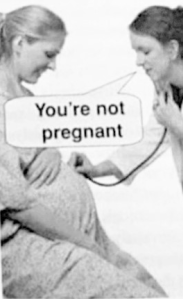
\includegraphics[width=0.2\textwidth]{images/13.png}
\end{center}


\item Na tabela a seguir estão os dados de diâmetro (mm) e peso (kg) de 10 amostras de rochas.

Dados:
\begin{center}
\begin{tabular}{|c|c|}
\hline
\textbf{Diâmetro (X)} & \textbf{Peso (Y)} \\
\hline
49 & 24,0 \\
65 & 40,0 \\
45 & 25,0 \\
40 & 23,5 \\
55 & 33,5 \\
45 & 22,0 \\
44 & 22,5 \\
47 & 23,5 \\
50 & 25,0 \\
56 & 35,0 \\
\hline
\end{tabular}
\end{center}
$\overline{X}=49,6$, $\overline{Y}=27,4$\\
$\sum_{i=1}^{10}X_{i}^{2}=25082$, $\sum_{i=1}^{10}Y_{i}^{2} = 7868$, $\sum_{i=1}^{10}X_{i}Y_{i} = 13978$\\
O coeficiente de determinação e a reta de ajuste de regressão linear são respectivamente:
\begin{enumerate}[A)]
    \item $r^{2}=0,9315;$
    \item $r^{2}=0,8677;$
    \item $r^{2}=-0,8677$
    \item $r=0,8677;$
    \item $r^{2}=0,8677; Y=12,627+0,807x$
\end{enumerate}

\item Uma nova unidade de dessalinização foi instalada em uma indústria química. Uma amostra com $n=10$, coletada antes da instalação da nova unidade indicou concentração de sal $\overline{x}_{1}=19,55$ e $s_{1}^{2}=15,35$ enquanto que, após a instalação, uma amostra com $n=16$ indicou $s_{2}^{2}=8,65$. Baseado nesses dados e utilizando $\alpha=0.05$
\begin{enumerate}[a)]
    \item teste a hipótese de que as duas variâncias sejam iguais;
    \item teste a hipótese de que a nova unidade reduziu a concentração média de sal.
\end{enumerate}

\item Os valores abaixo se referem aos pesos ao nascer (em kg) de bovinos da raça Ibagé, em duas épocas distintas:
Agosto: 18 25 16 30 35 23 21 33 32 22\\
Setembro: 27 30 20 30 33 34 17 33 20 23 39 23 28\\
Efetue o teste de homogeneidade de variâncias, ao nível $\alpha=0,05$.

\item Sabe-se que certa raça de bovinos em confinamento, alimentada com uma ração padrão, tem um aumento médio de peso igual a 60 kg durante os três primeiros meses de idade. Um lote de 10 novilhos, dessa mesma raça, recebeu um novo tipo de alimentação com novos concentrados. Mantendo-se as mesmas condições de manejo, os aumentos de peso foram 55; 62; 54; 58; 65; 65; 60; 62; 59; 67. Fixando o nível de significância em 1\%, conclua sobre o novo tipo de alimentação. Estime a média por intervalo e relacione o resultado com o teste de hipótese.

\item Para reduzir ambos os tipos de erro, devemos:
\begin{enumerate}[A)]
    \item acrescentar uma terceira hipótese ao teste
    \item aumentar o tamanho da amostra
    \item aumentar somente o nível de significância ($\alpha$)
    \item diminuir o tamanho da amostra
    \item aumentar o nível de confiança, ou seja, $1-\alpha$
\end{enumerate}

\item Para saber se uma determinada droga diminui, em média, a ação de bactérias no organismo, as hipóteses adequadas seriam:
\begin{enumerate}[A)]
    \item $H_0: \mu=\mu_{0}$, $H_1: \mu \neq \mu_{0}$
    \item $H_0: \mu=\mu_{0}$, $H_1: \mu > \mu_{0}$
    \item $H_0: \mu \neq \mu_{0}$, $H_1: \mu < \mu_{0}$
    \item $H_0: \mu=\mu_{0}$, $H_1: \mu < \mu_{0}$
    \item $H_0: \mu < \mu_{0}$, $H_1: \mu = \mu_{0}$
\end{enumerate}

\item Uma linha de produção opera com um peso médio de enchimento de 25ml por recipiente. O sobre enchimento e o subenchimento são problemas sérios e a linha de produção deve ser paralisada se qualquer um dos dois eventos ocorrer. Nesta situação, qual seria o teste mais adequado?
\begin{enumerate}[A)]
    \item $H_0: \mu=25$, $H_1: \mu \neq 25$
    \item $H_0: \mu=25$, $H_1: \mu > 25$
    \item $H_0: \pi=25$, $H_1: \pi \neq 25$
    \item $H_0: \mu \neq \mu_{0}$, $H_1: \mu = \mu_{0}$
    \item $H_0: \pi = \mu_{0}$, $H_1: \pi < \mu_{0}$
\end{enumerate}

\item Os dados a seguir correspondem à variável renda familiar e gasto com alimentação (em unidades monetárias) para uma amostra de 25 famílias.
\begin{center}
\begin{tabular}{|c|c|}
\hline
\textbf{Renda Familiar (X)} & \textbf{Gasto com Alimentação (Y)} \\
\hline
3 & 1,5 \\ 5 & 2,0 \\ 10 & 6,0 \\ 10 & 7,0 \\ 20 & 10,0 \\ 20 & 12,0 \\ 20 & 15,0 \\ 30 & 8,0 \\ 40 & 10,0 \\ 50 & 20,0 \\ 60 & 20,0 \\ 70 & 25,0 \\ 70 & 30,0 \\ 80 & 25,0 \\ 100 & 40,0 \\ 100 & 35,0 \\ 100 & 40,0 \\ 120 & 30,0 \\ 120 & 40,0 \\ 140 & 40,0 \\ 150 & 50,0 \\ 180 & 40,0 \\ 180 & 50,0 \\ 200 & 60,0 \\ 200 & 50,0 \\
\hline
\end{tabular}
\end{center}
\begin{center}
    % Nota: A URL original era um exemplo. Use um placeholder ou uma imagem local.
    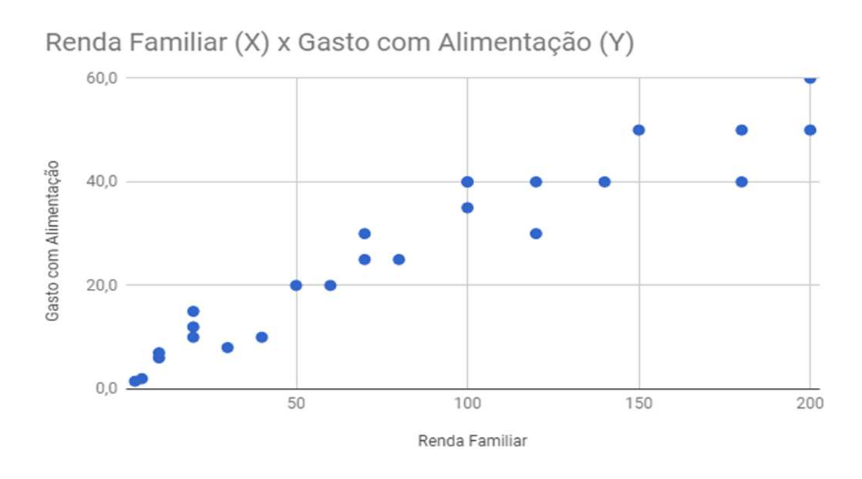
\includegraphics[width=0.625\textwidth]{images/21.png}
\end{center}
\begin{enumerate}[a)]
    \item Interprete o gráfico de dispersão e diga se o coeficiente de relação deve ser maior, igual ou menor do que zero.
    \item Calcule o coeficiente de correlação linear entre Renda Familiar(X) e Gasto com Alimentação(Y).\\
    Dados: $\overline{X}=83,12$, $\overline{Y}=26,66$\\
    $\sum_{i=1}^{25}X_{i}^{2}=271934$, $\sum_{i=1}^{25}Y_{i}^{2}=24899,25$, $\sum_{i=1}^{25}X_{i}Y_{i}=80774,5$
    \item Ajuste uma reta de regressão para a relação entre as variáveis Massa Muscular(Y) e Idade(X).
    \item Qual o significado prático do valor da inclinação da reta de regressão do item (c)?
\end{enumerate}

\item Um sofisticado simulador estocástico de tráfego fornece a velocidade média em avenidas de uma metrópole em função do volume de automóveis. O resultado de 14 simulações revelou o seguinte:
\begin{center}
\begin{tabular}{|c|c|}
\hline
\textbf{Volume de tráfego} & \textbf{Velocidade média} \\
\hline
3 & 95,6 \\ 3 & 93,8 \\ 5 & 74,4 \\ 5 & 74,8 \\ 10 & 50,5 \\ 10 & 51,5 \\ 15 & 44,6 \\ 15 & 42,4 \\ 20 & 35,8 \\ 20 & 38,7 \\ 25 & 32,0 \\ 25 & 3,2 \\ 30 & 30,1 \\ 30 & 29,1 \\
\hline
\end{tabular}
\end{center}
\begin{enumerate}[a)]
    \item Calcule o coeficiente de correlação linear de Pearson, interprete e teste sua significância a 5\%.
    \item Ajuste, teste e interprete o modelo de regressão linear simples.
\end{enumerate}

\item Uma pesquisa nacional indica que aproximadamente 25\% das contas de grandes magazines incorrem em penalidade por atraso nos pagamentos. Se um magazine local constata 40 atrasos numa amostra de 200 clientes, pode necessariamente admitir que seus clientes sejam melhores que os clientes de todo país? Adote 5\% de significância.

\item Um fabricante de conservas anuncia que o conteúdo líquido das latas de seu produto é, em média, 50 gramas. A fiscalização desconfia que as gramas estão abaixo do especificado pelo fabricante. Para testar esta hipótese, utilizando uma amostra aleatória de 180 latas, o teste mais adequado seria:
\begin{enumerate}[A)]
    \item $H_0: \mu=50$, $H_1: \mu \neq 50$
    \item $H_0: \mu=180$, $H_1: \mu < 180$
    \item $H_0: \mu=50$, $H_1: \mu < 180$
    \item $H_0: \mu=180$, $H_1: \mu < 50$
    \item $H_0: \mu=50$, $H_1: \mu < 50$
\end{enumerate}

\item Supondo-se que o fabricante está realmente vendendo o seu produto com as gramas abaixo do especificado (questão 24), mas o fiscal decide por não o autuar, que tipo de erro pode estar sendo cometido?

\item Os dados abaixo referem-se aos pesos iniciais e ganhos de peso (em gramas) de 15 ratos fêmeas entre 24 a 84 dias de idade, submetidas a uma dieta com altos teores de proteína. O objetivo deste estudo é verificar se o ganho de peso está relacionado com o peso inicial. Sendo assim, experimentos de alimentação podem ser mais precisos, levando-se em conta o peso inicial dos ratos, ou fazendo-se o pareamento ou ainda por ajustes de diferenças no peso inicial.
\begin{enumerate}[a)]
    \item Calcule o coeficiente de correlação linear de Pearson, interprete e teste sua significância a 5\%.
    \item Ajuste, teste e interprete o modelo de regressão linear simples.
\end{enumerate}
\begin{center}
\begin{tabular}{|c|c|c|}
\hline
\textbf{Ratos} & \textbf{Peso inicial} & \textbf{Ganho de peso} \\
\hline
1 & 50 & 12 \\
2 & 64 & 15 \\
3 & 76 & 15 \\
4 & 64 & 11 \\
5 & 74 & 13 \\
6 & 60 & 11 \\
7 & 69 & 96 \\
8 & 68 & 12 \\
9 & 56 & 13 \\
10 & 57 & 11 \\
11 & 48 & 10 \\
12 & 59 & 10 \\
13 & 46 & 82 \\
14 & 45 & 10 \\
15 & 65 & 10 \\
\hline
\end{tabular}
\end{center}

\item Diante de uma equipe de fiscais, a nutricionista responsável pelo cardápio de um restaurante declarou que o peso médio de uma determinada vitamina por bandeja de refeição é de 5,5 g. Foi retirada uma amostra de 25 bandejas do fornecimento diário de refeições desse restaurante, encontrando-se uma média de 5,2 g da vitamina e um desvio padrão de 1,2 g. Verifique a veracidade da informação da nutricionista, utilizando nível de significância de 5\%.

\item O Instituto de Nutrição da América Central e Panamá fez um estudo intensivo de resultados de dietas publicados em revistas científicas. Uma dieta aplicada a 15 pessoas produziu os seguintes níveis de colesterol (em $mg/l$): 204; 108; 140; 152; 158; 129; 175; 146; 157; 174; 192; 194; 144; 152; 135. Sabendo-se que o nível médio normal de colesterol é de $190~mg/l$, verifique se a redução no teor médio de colesterol das pessoas submetidas a essa dieta foi significativa, com $\alpha=0,05$.

\item Em geral, experimentos afirmam que a percentagem de frutos atacados por larvas de mariposa é maior em macieiras anãs. Aparentemente, a densidade de mariposas não tem relação com o tamanho do pomar ou porte da planta, de modo que os riscos de ataque em um fruto em particular seriam aumentados quando o número de frutos ou plantas for pequeno. Os dados abaixo se referem aos resultados de um experimento contendo evidências sobre esse fenômeno.
\begin{enumerate}[a)]
    \item Calcule o coeficiente de correlação linear de Pearson, interprete e teste sua significância.
    \item Ajuste, teste e interprete o modelo de regressão linear simples.
\end{enumerate}
\begin{center}
% The table will now occupy the full text width
\begin{tabularx}{\textwidth}{|c|>{\Centering}X|>{\Centering}X|}
\hline
\textbf{Plantas} & \textbf{Tamanho da colheita (centenas de frutos)} & \textbf{Percentagem de frutos atacados} \\
\hline
1 & 8 & 59 \\
2 & 6 & 58 \\
3 & 11 & 56 \\
4 & 22 & 53 \\
5 & 14 & 50 \\
6 & 17 & 45 \\
7 & 18 & 43 \\
8 & 24 & 42 \\
9 & 19 & 39 \\
10 & 23 & 38 \\
11 & 26 & 30 \\
12 & 40 & 27 \\
\hline
\end{tabularx}
\end{center}

\item É esperado que a massa muscular de uma pessoa diminua com a idade. Para estudar essa relação, uma nutricionista selecionou 18 mulheres, com idade entre 40 e 79 anos, e observou em cada uma delas a idade (X) e a massa muscular (Y).
\begin{center}
\begin{tabular}{|c|c|}
\hline
\textbf{Massa muscular (Y)} & \textbf{Idade (X)} \\
\hline
100.0 & 43 \\
116.0 & 45 \\
97.0 & 45 \\
105.0 & 49 \\
100.0 & 53 \\
87.0 & 56 \\
80.0 & 56 \\
76.0 & 58 \\
91.0 & 64 \\
84.0 & 65 \\
68.0 & 67 \\
78.0 & 68 \\
78.0 & 68 \\
82.0 & 71 \\
73.0 & 73 \\
73.0 & 73 \\
65.0 & 76 \\
77.0 & 78 \\
\hline
\end{tabular}
\end{center}
Dados: $\overline{X}=61,556$, $\overline{Y}=85$\\
$\sum_{i=1}^{18}X_{i}^{2}=70362$, $\sum_{i=1}^{18}Y_{i}^{2}=133300$, $\sum_{i=1}^{18}X_{i}Y_{i}=91964$\\
O coeficiente de correlação linear e a reta linear que melhor se ajusta ao modelo é:
\begin{enumerate}[A)]
    \item $r=0,837; Y=-148,218-1,027x$
    \item $r=-0,837; Y=148,218+1,027x$
    \item $r^{2}=-0,837; Y=148,218-1,027x$
    \item $r=0,837; Y=148,218-1,027x$
    \item $r=-0,837; Y=148,218-1,027x$
\end{enumerate}

\item Uma organização médica afirma que um novo medicamento é de qualidade superior ao medicamento até então existente no mercado. A organização afirma que a nova medicação é 80\% mais eficaz. Examinada uma amostra de 200 pacientes, verificou-se que 120 deles ficaram curados com o novo tratamento. O teste mais adequado neste caso seria:
\begin{enumerate}[A)]
    \item $H_0: \pi = 0.80$, $H_1: \pi \neq 0.80$
    \item $H_0: \pi=0.80$, $H_1: \pi > 0.80$
    \item $H_0: \pi=120$, $H_1: \pi > 120$
    \item $H_0: \mu=0.80$, $H_1: \mu > 0.80$
    \item $H_0: \mu=120$, $H_1: \mu > 120$
\end{enumerate}

\item Para testar a performance em termos de consumo de combustível de um novo carro compacto, o fabricante sorteou seis motoristas profissionais que dirigiram o automóvel de Pelotas a Porto Alegre. O consumo do carro (em litros) para cada um dos seis motoristas foi de 27,2; 29,3; 31,5; 28,7; 30,2; 29,6. Baseado nesses dados e utilizando nível de significância de 5\%, o fabricante pode indicar que o consumo médio do novo carro é de 30 litros para viagens nesse percurso?

\item O dono de uma loja de materiais de construção denunciou seu fabricante de parafusos afirmando que este coloca no mercado uma quantidade de unidades defeituosas que supera os 20\% da quantidade total. Uma investigação foi conduzida com uma amostra aleatória de 50 unidades, das quais 28\% acusaram defeito. Você diria que a investigação fundamenta esta denúncia? Use 10\% de significância.

\item Vinte observações de um tipo de matriz indicaram um tempo de vida média de 217 minutos desvio padrão de 20 minutos. Teste a hipótese de que o tempo de vida é inferior a 250 minutos, conforme atestam alguns engenheiros. Use $\alpha=0,05$.

\item Supondo-se que a medicação nova na verdade não é mais eficaz que a atual (questão 31), porém os examinadores decidiram investir na nova medicação (menos eficaz), que tipo de erro pode estar sendo cometido? Justifique.

\item Os dados a seguir representam o ganho obtido em um processo químico. Use $\alpha=0,05$ e teste a hipótese de que nas condições atuais o ganho seja superior a 1,5.
\begin{center}
\begin{tabular}{|c|c|c|c|c|c|c|c|}
\hline
1,50 & 1,55 & 1,59 & 1,42 & 1,53 & 1,58 & 1,48 & 1,52 \\
\hline
1,53 & 1,62 & 1,46 & 1,56 & 1,63 & 1,54 & 1,58 & 1,68 \\
\hline
\end{tabular}
\end{center}

\item Um engenheiro desconfia que o percentual de produtos defeituosos reduziu depois da implantação do controle estatístico de processo (CEP). Em uma amostragem de 500 produtos realizada antes da implantação do CEP, identificou-se 5 produtos defeituosos. Após a implantação do CEP, coletou-se uma amostra de 700 produtos e identificou-se um defeituoso. Teste a hipótese do engenheiro usando 2,5\% de significância e enuncie que pressuposto você estaria infringindo para utilizar o teste Z.

\item Dois tipos de combustíveis estão sendo testados. A hipótese é que eles tenham o mesmo desempenho. Teste essa hipótese, sabendo que os resultados de testes feitos com 10 automóveis usando cada tipo combustível indicaram $s_{1}=0,63~km/l$ e $s_{2}=0,88~km/l$ e $\overline{x}_{1}=13,3~km/l$ e $\overline{x}_{2}=13,9~km/l$. (Suponha $\sigma_{1}^{2}=\sigma_{2}^{2}$ e use $\alpha=0,05$).

\item Para investigar se o treinamento é ou não transferido pelo ácido nucléico, 10 ratos foram treinados em discriminar se havia luz ou escuridão. Posteriormente esses ratos foram mortos, o ácido nucléico extraído e injetados em 10 ratos. Simultaneamente o ácido nucléico de 10 ratos não treinados foram injetados em outros 10. Os 20 ratos foram observados durante um período e o número de erros relativos a cada rato está na tabela abaixo. Verifique se, em média, os ratos treinados erram tanto quanto os ratos não treinados. (Suponha $\sigma_{1}^{2}=\sigma_{2}^{2}$ e use $\alpha=0.05$).
\begin{center}
\begin{tabular}{|c|c|}
\hline
\textbf{Treinado} & \textbf{Não treinado} \\
\hline
7 & 12 \\
9 & 8 \\
6 & 9 \\
11 & 13 \\
13 & 14 \\
8 & 9 \\
7 & 8 \\
13 & 10 \\
12 & 7 \\
9 & 15 \\
\hline
\end{tabular}
\end{center}

\item Em uma indústria química, os engenheiros desejam saber se o alongamento (cm) de um composto de borracha permanece inalterado ao passar por uma máquina extrusora. Como o alongamento do composto depende do lote de matéria-prima usado na sua confecção, os dados foram coletados aos pares. A que conclusão se pode chegar a partir desses dados, com $\alpha=0,05$?
\begin{center}
\begin{tabular}{|c|c|c|}
\hline
\textbf{Lote} & \textbf{Antes} & \textbf{Depois} \\
\hline
1 & 360 & 360 \\
2 & 370 & 365 \\
3 & 380 & 355 \\
4 & 345 & 340 \\
5 & 365 & 350 \\
6 & 380 & 370 \\
7 & 390 & 390 \\
8 & 395 & 375 \\
9 & 385 & 375 \\
10 & 410 & 395 \\
\hline
\end{tabular}
\end{center}

\item Um engenheiro deseja testar a hipótese de que o percentual de peças defeituosas é inferior a 10\%. Uma amostra aleatória com 75 peças revelou 6 peças defeituosas. Use $\alpha=0.05$ e conclua a respeito.

\item Os dados abaixo dão os acertos obtidos por oito soldados num experimento destinado a determinar se a precisão do tiro é afetada pela maneira de dispor os olhos: com o olho direito aberto ou com o olho esquerdo aberto. Que conclusão você poderia tirar, com $\alpha=0,05$?
\begin{center}
\begin{tabular}{|c|c|c|}
\hline
\textbf{Soldado} & \textbf{Direito} & \textbf{Esquerdo} \\
\hline
1 & 44 & 40 \\
2 & 39 & 37 \\
3 & 33 & 28 \\
4 & 56 & 53 \\
5 & 43 & 48 \\
6 & 56 & 51 \\
7 & 47 & 45 \\
8 & 58 & 60 \\
\hline
\end{tabular}
\end{center}

\item Um fabricante alega que apenas 2\% das peças que ele fornece estão abaixo das condições de utilização. Em 200 peças escolhidas aleatoriamente de uma remessa de 5.000 encontraram-se 10 falhas. A alegação do fabricante parece aceitável ao nível de 5\% de significância?

\item Cinco medidas do conteúdo de alcatrão em um cigarro X acusaram: 14,5, 14,2, 14,4, 14,8, e 14,1 miligramas por cigarro. Este conjunto de cinco valores tem média 14,4 e desvio padrão 0,274. O leitor pretende testar a hipótese nula $H_0: \mu=14,1$ (conforme declarado no maço) ao nível de 0,05 de significância.
\begin{enumerate}[a)]
    \item $H_{0}$ seria aceita, contra a alternativa $H_{A}: \mu \neq 14,1?$
    \item $H_{0}$ seria aceita, contra a alternativa $H_{A}: \mu < 14,1?$
    \item $H_{0}$ seria aceita, contra a alternativa $H_{A}: \mu > 14,1?$
    \item Que suposições são necessárias para fazer o teste de hipóteses?
\end{enumerate}

\item Suponha que um fabricante sem escrúpulos deseje uma "prova científica" de que um aditivo químico totalmente inócuo melhora o rendimento.
\begin{enumerate}[a)]
    \item Se um grupo de pesquisa analisa esse aditivo com um experimento, qual é a probabilidade de chegar a um "resultado significativo" com $\alpha=0,05$ (para promover o aditivo com "afirmações científicas") mesmo que o aditivo seja totalmente inócuo?
    \item Se dois grupos independentes de pesquisa analisam o aditivo, qual é a probabilidade de que pelo menos um deles chegue a um "resultado significativo", mesmo que o aditivo seja totalmente inócuo?
    \item Se 32 grupos independentes de pesquisa analisam o aditivo, qual é a probabilidade de que pelo menos um deles chegue a um "resultado significativo", mesmo que o aditivo seja totalmente inócuo?
\end{enumerate}

\item Suponha que um farmacêutico pretenda achar um novo unguento para reduzir inchação. Para tanto, ele fabrica 20 medicamentos diferentes e testa cada um deles, ao nível de 0,10 de significância, quanto a finalidade em vista. Qual a probabilidade de ao menos um deles "se revelar" eficaz mesmo que todos sejam totalmente inócuos?

\item Um médico está estudando o crescimento de dois tipos de bactérias. Como pode haver um efeito significativo do substrato, os dois tipos de bactérias foram cultivados em cada uma das oito amostras de substrato. Use $\alpha=0,01$ e teste a hipótese de que a bactéria 1 cresce mais que a bactéria 2.
\begin{center}
\begin{tabular}{|c|c|c|}
\hline
\textbf{Substrato} & \textbf{Bactéria 1} & \textbf{Bactéria 2} \\
\hline
1 & 3,0 & 3.2 \\
2 & 3,2 & 3,1 \\
3 & 2,7 & 2.4 \\
4 & 2,5 & 2,1 \\
5 & 3,8 & 3,2 \\
6 & 4,3 & 3,7 \\
7 & 3,5 & 3,2 \\
8 & 4,8 & 4,0 \\
\hline
\end{tabular}
\end{center}

\end{enumerate}

\hrulefill

\section*{GABARITO}

\begin{enumerate}
    \item $f_{0,025}=4,03$; $f_{\text{calc}}=5$; Pode-se considerar a desigualdade de variâncias; $t_{0,025}=2,179$; $t_{\text{calc}}=1,471$; Não se rejeita $H_0$.
    \item 
    \begin{enumerate}[a)]
        \item V
        \item F: a hipótese estatística é uma suposição feita a respeito de um ou mais parâmetros, como, por exemplo, média populacional e a proporção populacional.
        \item V
        \item F: Quando não temos motivos suficientes para supor que uma das médias será maior que a outra, formulamos uma hipótese alternativa bilateral (mais genérica).
        \item V
        \item F: evitou-se o erro tipo I, ou seja, culpá-lo sendo ele inocente (considerando $H_0$: inocente)
        \item V
        \item F: o juiz cometeu o erro tipo II, ou seja, inocentá-lo quando era culpado (considerando $H_0$: inocente).
    \end{enumerate}
    \item 
    \begin{enumerate}[a)]
        \item $r=0,8015$; $t_{\text{calc}}=3,791$; $t_{0,025}=2,306$; Rejeita-se $H_0$.
        \item $Y=3+0,475 X$
    \end{enumerate}
    \item 
    \begin{enumerate}[a)]
        \item $r=0,9830$; $t_{\text{calc}}=11,978$; $t_{0,025}=2,571$; Rejeita-se $H_0$.
        \item $Y=11,13+0,13 X$
    \end{enumerate}
    \item Pressupõe-se que a variável em estudo tem distribuição normal e que as amostras retiradas das populações são independentes nos casos em que as variâncias $Var_1$ e $Var_2$ são conhecidas, mas supostas iguais ou ainda desconhecidas e desiguais.
    \item Os erros estão relacionados a má decisão tomada referente a hipótese testada. Estamos sujeitos a rejeitar algo que estava adequado e aceitar uma hipótese alternativa (erro tipo I) ou não rejeitar algo que está ruim e descartar uma hipótese alternativa (erro tipo II). O mais grave seria tomar a decisão de trocar algo certo por algo errado, ou seja, o erro tipo I.
    \item Letra D
    \item $f_{0,025}=5,82$; $f_{\text{calc}}=1,137$; Pode-se considerar a igualdade de variâncias; $t_{0,025}=2,179$; $t_{\text{calc}}=-0,953$; Não se rejeita $H_0$.
    \item
    \begin{enumerate}[a)]
        \item $r=-0,7732$; $t_{\text{calc}}=-5,718$; $t_{0,025}=2,074$; Rejeita-se $H_0$.
        \item $Y=185,96-2,09 X$
    \end{enumerate}
    \item
    \begin{enumerate}[a)]
        \item $f_{0,025}=3,72$; $f_{\text{calc}}=3,624$; Pode-se considerar a igualdade de variâncias.
        \item $t_{0.05}=-1,725$; $t_{\text{calc}}=-32,204$ (teste unilateral); Rejeita-se $H_{0}$.
    \end{enumerate}
    \item $t_{0.025}=2,365$; $t_{\text{c}}=-3,161$; Rejeita-se $H_{0}.$
    \item
    \begin{enumerate}[a)]
        \item $f_{0,025}=7,39$; $f_{\text{calc}}=2,020$; Pode-se considerar a igualdade de variâncias.
        \item $t_{0,025}=2,262$; $t_{\text{calc}}=-1,528$; Não se rejeita $H_{0}$.
    \end{enumerate}
    \item Erro tipo I. Sendo $H_0$: está grávida e $H_1$: não está grávida, neste caso, não se rejeita a hipótese nula, uma vez que a paciente está grávida. Ao se optar pela hipótese alternativa, a médica está afirmando que a sua paciente não está grávida, ou seja, está cometendo o erro tipo I (Rejeitar a hipótese nula, quando deveria aceitá-la).
    \item Letra B
    \item 
    \begin{enumerate}[a)]
        \item $f_{0,025}=3,12$; $f_{\text{calc}}=1,775$; Pode-se considerar a igualdade de variâncias.
        \item $t_{0,05}=1,711$; $t_{\text{calc}}=1,2622$ (teste unilateral); Não se rejeita $H_0$.
    \end{enumerate}
    \item $f_{0.05}=3.44$; $f_{\text{calc}}=1,0289$ (teste bilateral); Não se rejeita $H_0$.
    \item $t_{0,005}=3,250$; $t_{c}=0,5121$; Não se rejeita $H_0$. Intervalo para a média (56,26; 65,14). Como o valor 60 está contido no intervalo, chega-se a mesma conclusão do teste.
    \item Letra B
    \item Letra D
    \item Letra A
    \item 
    \begin{enumerate}[a)]
        \item r>0;
        \item $r=0,954$
        \item $Y=5,38+0,256x;$
        \item O valor 0,256 significa que estima-se que para cada aumento de uma unidade monetária da renda familiar ocorre um acréscimo em média de 0,256 unidades no gasto com alimentação.
    \end{enumerate}
    \item
    \begin{enumerate}[a)]
        \item $r=-0,8893$; $t_{\text{calc}}=-6,735$; $t_{0,025}=2,179$; Rejeita-se $H_0$.
        \item $Y=86,73-2,40 X$
    \end{enumerate}
    \item $z_{0.025}=-1,96$; $Z_{\text{calc}}=-1,6330$; Não se rejeita $H_0$.
    \item Letra E
    \item Erro Tipo II. Aceitar a hipótese nula, quando deveria rejeitá-la.
    \item
    \begin{enumerate}[a)]
        \item $r=0,4894$; $t_{\text{calc}}=2,024$; $t_{0,025}=2,160$; Não se rejeita $H_{0}$.
        \item $Y=54,95+1,06 X$
    \end{enumerate}
    \item $t_{0,025}=2,064$; $t_{c}=-1,25$; Não se rejeita $H_0$.
    \item $t_{0,05}=-1,761$; $t_{c}=-4,803$ (teste unilateral); Rejeita-se $H_0$.
    \item
    \begin{enumerate}[a)]
        \item $r=-0,8809$; $t_{\text{calc}}=-5,884$; $t_{0,05}=2,228$; Rejeita-se $H_0$.
        \item $Y=64,25-1,01x$
    \end{enumerate}
    \item Letra E
    \item Letra B - O parâmetro a ser testado é a proporção ($\pi$)
    \item $t_{0,025}=2,571$; $t_{c}=-0,989$; Não se rejeita $H_{0}$.
    \item $Z_{0,1}=1,28$; $Z_{\text{calc}}=1,41$ (teste unilateral); Rejeita-se $H_{0}$.
    \item $t_{0,25}=-1,729$; $t_{c}=-7,379$ (teste unilateral); Rejeita-se $H_{0}.$
    \item Erro Tipo I. Rejeitar a hipótese nula, quando deveria aceitá-la.
    \item $t_{0,25}=1,753$; $t_{c}=2,909$ (teste unilateral)
    \item $z_{0.05}=1,96$; $Z_{\text{calc}}=1,834$ (teste unilateral); Não se rejeita $H_0$. Aproximação normal não é satisfatória, pois $np \le 5$, antes e depois do CEP.
    \item $t_{0,025}=-2,101$; $t_{c}=-1,753$; Não se rejeita $H_0$.
    \item $t_{0,025}=2,101$; $t_{c}=-0,829$; Não se rejeita $H_0$.
    \item $t_{0,025}=2,262$; $t_{c}=3,9925$; Rejeita-se $H_{0}$ (TH para amostras pareadas)
    \item $Z_{0,025}=-1,64$; $z_{\text{calc}}=-0,5714$ (teste unilateral); Não se rejeita $H_0$.
    \item $t_{0.025}=2,365$; $t_{c}=7.03$; Rejeita-se $H_{0}$. (TH para amostras pareadas)
    \item $Z_{0,025}=1,96$; $Z_{\text{calc}}=3,0305$; Rejeita-se $H_0$.
    \item
    \begin{enumerate}[a)]
        \item $t_{0,025}=2,776 \Rightarrow H_{0}$ é aceita, a média não é significativamente diferente de 14,1.
        \item $t_{0,05}=-2,132 \Rightarrow H_{0}$ é aceita, não é possível afirmar que a média é menor que 14,1.
        \item $t_{0,05}=2.132 \Rightarrow H_{0}$ é rejeitada, a média deve ser maior que 14,1.
        \item A variável em estudo tem distribuição normal
    \end{enumerate}
    \item
    \begin{enumerate}[a)]
        \item $5\%=P(\text{erro Tipo I})$
        \item 0,0975
        \item 0,8063
    \end{enumerate}
    \item 0,8784
    \item $t_{0,005}=2,998$; Não se rejeita $H_{0}$. $t_{\text{calc}}=0,9534$ (teste unilateral)
\end{enumerate}

\end{document}